\documentclass{ltjsbook}
\usepackage{docmute} 
\usepackage{../../myStyle} 

\begin{document}
\setcounter{chapter}{5}
\chapter{社会心理学の歴史5;社会心理学の発展，転換，混沌期}
\label{sp06_history3}
\section{転換期への序説}
それでは時間になりましたので，社会心理学\index[termidx]{しゃかいしんりがく@社会心理学}の話を始めようと思います。今日は地声で喋ろうと思います。十分聞こえますよね。静かな部屋なので，この感じでやらせてもらえたらと思います。

今日は第6回になります。本来であれば，今日でもって「歴史シリーズ」「第1部完」，というところになるかなと思うんですが，授業の準備やレジメ等の準備をしていて思うに，ひょっとしたら中途半端なところで終わってしまいそうです。そのため，次回にもう一つお話を追加することになるかもしれませんが，基本的にほぼ現代のところまで時計を進めていきたいと思っています。

前回社会心理学\index[termidx]{しゃかいしんりがく@社会心理学}が成立した時期の一つとして，1935年の社会心理学\index[termidx]{しゃかいしんりがく@社会心理学}ハンドブックの発刊をひとつの区切りにしましょう，という話をしましたよね。今日はそこから50年，60年くらい進んで，21世紀に入るぐらいのところまでいけたらなと思っています。次回は，そういう意味では歴史というよりは現代のお話に行きますので，メインのお話としてはここで一旦，第一部は終わると思います。次回も歴史的な話をしますが，一旦ここで過去の話は今日で終わるかなと思っています。

\section{前回の振り返り}

前回の講義を振り返っておきたいと思います。特に強調したのは，モレノのソシオメトリーとレヴィンの場の理論という2つの理論でした。

モレノのソシオメトリーについては，関連してホーソン実験もご紹介しました。これは産業心理学や産業社会学でよく触れられる研究です。モレノのソシオメトリーは，人間関係を多角的に測定しようという試みでした。当時の測定技術には限界がありましたが，その多角的な計測を基に，集団療法やグループワークのカウンセリングを実践していこうという動きがありました。

モレノは，集団療法，ソシオメトリー，サイコドラマ(即興劇)という分野で，今でも臨床心理学の領域でその考え方が生きています。ただ，社会心理学\index[termidx]{しゃかいしんりがく@社会心理学}にはあまり残っておらず，コールドソシオメトリー，つまり測定法としてのソシオメトリーだけが入ってきたような状況です。教育現場でも導入されたのですが，教育上のいろいろな問題があって禁止されてしまいましたからね。

ホーソン実験は，工場で7年もかけて行われた大規模な実験です。物理的な環境の調整や給与体系の調整，運用上の調整をして，パフォーマンスを上げるにはどうしたらよいのかという関数関係を探ろうとしました。科学的な管理運営を目指したのですが，結局キーとなったのは，目に見える関係ではなく，インフォーマルな人間関係だったんです。この，科学的にコントロールしようという発想と，そこからこぼれ落ちるものをどう拾い上げるかという課題から，心理学的・解釈的アプローチの必要性が認識され，社会心理学\index[termidx]{しゃかいしんりがく@社会心理学}的な学術テーマを考える土壌が形成されました。

その後，社会心理学\index[termidx]{しゃかいしんりがく@社会心理学}は「現実問題に対応できる学問です」「政策に使える」「意思決定に活用できる」という形でアメリカで展開されていきました。多くのユダヤ人研究者がアメリカに亡命したこともあり，アメリカ固有の個人主義やプラグマティズムという風土と融合して，人間の行動を科学的に研究する，とてもモダーンなサイエンスが確立されていったのです。

ヨーロッパの方ではゲシタルト心理学が流行っていたわけですが，その一波としてアメリカに来たレヴィンたちがグループダイナミックス\index[termidx]{ぐるーぷだいなみっくす@グループダイナミックス}研究所を作りました。彼の提唱した場の理論は，集団力学\index[termidx]{しゅうだんりきがく@集団力学}という新しい学問を生み出したというお話をしました。

\section{転換期，再生期あるいは混沌期のはじまり}

さて，1935年から50年くらいの間に社会心理学\index[termidx]{しゃかいしんりがく@社会心理学}がしっかりと形を成し，一つの学問として確立したところまで説明しました。今日はそこから2000年にかけての動きについてお話ししたいと思います。テキスト\parencite{anatomia}の「アナトミア社会心理学\index[termidx]{しゃかいしんりがく@社会心理学}」も6章の後半に入っていまして，この本では1960年代前半から現代にかけての時期を，社会心理学\index[termidx]{しゃかいしんりがく@社会心理学}の転換期あるいは再生期と名付けています。

転換期あるいは再生期，別の言い方では混沌とした時代，混沌期とも書いてあります。つまり，成立した後，変わっていく，あるいは別の形に変わっていく，でもいろんなものが混ざり合って変わっていくという意味で，そういった名前が付いているわけですが，どういった考え方があって，その様々な学派が出てきたのか，あるいはどういったところで混沌としているという話になったのかということを今日は解説していきたいと思います。

この本が出たのが2002年，21世紀になってまもなく2002年の2月に出ていますから，執筆をしたのはおそらく2000年，2001年に入ったところだと思うわけです。吉森先生の考え方において，再生期というのは多分その辺の発想が入っているんじゃないかと思います。この本は社会的構築主義という話の方向に割と重点を置いているような気がします。これは私の個人的な感想ですが。

第7章は，2000年までのこの話を受けて，これからも社会心理学\index[termidx]{しゃかいしんりがく@社会心理学}はまだまだ発展していくのでよろしく！というような形で締めくくられているわけですが，その方向性というのも，どちらかというと，社会的構築主義に基づく，そういった感じの社会心理学\index[termidx]{しゃかいしんりがく@社会心理学}ですね。社会的構築主義，ナラティブ的なもの，今日ご紹介するガーゲン\index[nameidx]{がーげん@ガーゲン}的な感じの社会心理学\index[termidx]{しゃかいしんりがく@社会心理学}という方向に広がるんじゃないかというのが，この本の主張です。

突然の自己紹介で恐縮ですが，私が大学生になったのが1994年です。大学院生になったのが98年，ドクターコースに入ったのがミレニアムの2000年，ジャストの年でございます。

というわけで，今日お話しする時代は私の若い頃と重なります。吉森先生とは異なる視点から，同時代を生きた者としての話も少し加えてお話ししたいと思います。年配者の昔話は若い方には退屈かもしれませんが，過去の事例として聞いていただければと思います。これも20年以上前のことですからね。これを踏まえて，現代の展開や今後の方向性，そして社会心理学\index[termidx]{しゃかいしんりがく@社会心理学}とは何かということを考えていっていただきたいと思います。

\subsection{1960年代の時代背景}
では，1935年頃に基盤が確立し，社会心理学\index[termidx]{しゃかいしんりがく@社会心理学}という学問が本格的に始まってから少し経った1960年代からお話を始めましょう。60年代は第二次世界大戦後の時期です。日本は敗戦を経験し，世界的に見ても帝国主義の時代は終わり，冷戦の時代へと移行していく時期でした。この授業で何度も強調しましたが，20世紀初頭の科学の発展は目覚ましく，「20世紀は物理学の世紀」とも言われます。科学の急速な発展は第一次，第二次世界大戦を経て，最終的に日本への原爆投下という事態を招きました。物理学の発展により，人類は地球を破壊しうる科学力を手に入れたわけです。太平洋戦争後，冷戦という緊張状態の中で，20世紀前半の科学万能主義的な考え方に疑問が投げかけられるようになりました。

その背景には環境問題の顕在化がありました。工場の増加や大量消費の弊害が明らかになり，資本主義的な利益追求が環境に及ぼす影響への懸念が高まりました。アメリカではベトナム戦争への批判も強まり，科学の進歩が生活を豊かにする一方で，その方向性を問い直す反省的な機運が生まれてきました。ヒッピー族の出現に象徴されるように，反科学的なムーブメントも起こってきたのです。

\subsection{認知革命の影響}

学問の世界では，認知革命\index[termidx]{にんちかくめい@認知革命}が起きていました。認知心理学\index[termidx]{にんちしんりがく@認知心理学}が台頭してきたのです。1913年にワトソン\index[nameidx]{わとそん@ワトソン}が行動主義を宣言し，刺激(S)と反応(R)の連合による客観的な科学を提唱しましたが，「SとRだけでなく，その間をつなぐ有機体のことも考える必要がある」という認識から認知心理学\index[termidx]{にんちしんりがく@認知心理学}が発展しました。この「認知」という概念は非常に重要で，その背景にはコンピューターの発展がありました。

第二次大戦を経て，コンピューターは非常に発展していきました。私が物心ついた1980年頃には，ファミリーコンピューターというゲーム機が家庭に普及する時代がありました。その頃は，ファミコンやパソコンとは言わず，マイコンと呼んでいました。パーソナルコンピューターではなく，マイコンピューター，つまり私のコンピューターだったんです。その前の60年代，70年代は大型計算機の時代でした。東大や京大などに大型計算機センターが設立され，計算機を用いて計算をする時代だったんです。その大型計算機が次第に小さくなり，現在のノートパソコン，ラップトップのサイズまで縮小していくんですね。

ちなみに，私が94年に大学生になった年。私は関西大学に在籍していました。当時の情報処理の授業では，TSSという大型コンピューターに接続して統計分析をすることを学びました。それが基本でした。TSSというのは，タイムシェアリングシステム，つまり自分の番を待つシステムのことを指します。これは，関西大学の情報処理センターにあるスパコン，大型計算機の計算力が非常に高いため，全員が同時にアクセスしても，それぞれの計算タスクを順番にミリセカンド単位で処理していくので，ユーザ側はほとんどリアルタイムで，ユーザが計算をさせているような感覚で使える，というものです。これが大型計算機の時代だったんです。

しかし，私が94年に大学生になった時，この使い方を学んだものの，その翌年にはWindows95が登場しました。つまり，パソコンの時代が来たわけです。その1年間，TSSも多分もう終わりかけだったと思いますが，徐々にパソコンの時代が訪れました。サイズが小さくなって，頑張ればデスクトップパソコンが一人一台使えるようになりました。大型のコンピューターに預けていた脳みそを自分のものにすることができるようになった，というのが90年代の状況です。

話が逸れましたが，ともかく60年代，70年代にはコンピューターが発展してきました。大型計算機，真空管の時代からICチップ，集積回路になり，さらにスーパーLSIになっていきました。そうした進歩により，多くの計算が可能になりました。

その計算をする際，ハードウェアの仕組みは同じでも，ソフトウェアによって計算を様々に変えられる「ノイマン型の発想のコンピューター」の登場により，「ハードウェア」と「ソフトウェア」という発想が生まれました。皆さんには当たり前に聞こえるかもしれませんが，ハードとソフトの区別を私が初めて知ったのは，ファミコンのようなゲームが出てきてからの話です。

皆さんはソフトと言えばスマホにインストールするものと思うかもしれません。でも私が子供の頃，「ファミコン買って」と親に言うと，「ゲームは一つしかできないじゃないか。次のゲームが欲しくなったらどうするんだ」と言われたものです。ファミコン以前は，このテキストの半分ほどのサイズで開くゲームウォッチという携帯型ゲーム機がありました。それは，ドンキーコングならドンキーコングというソフトが入ったハードそのものでした。違うゲームがしたければ，新しいハードを買う必要があったんです。でも，ファミリーコンピューターは違いました。カセットを変えるだけでゲームが変わるんです。

つまり「本体を買えば，ソフトを買い換えるだけでいろんなゲームができる」という概念が一般に浸透してきたのが80年代頃だということです。コンピューターの登場とともに，「ハードウェア」と「ソフトウェア」を分離する考え方が生まれ，一般的になったのです。

これが当然，心理学的な考え方にも応用されてきます。「人間も，体は違えども，体の問題と心の問題がある。体はハードウェアで，心はソフトウェアだ」という見立てです。人間の心をコンピューターのように考えると，心はハードウェアの制限を受けつつも，かなり多様なことができるようになっています。

私たちは映画を楽しんだり，音楽を楽しんだり，本を楽しんだり，様々な精神活動をします。これは，様々なアプリケーションが走っているようなイメージですね。ソフトでいろんなアプリケーションが動いている。その本体には意識というOSがあって，そのOSは体の調子にも影響され，また制御してもいる。体の感覚，内受容感覚などはもっと下のレベルで，BIOSがコントロールしている\footnote{BIOS(Basic Input/Output System)は，コンピュータの起動時に基本的なハードウェアの初期化とシステムの起動を行うハードウェアとソフトウェアの中間に位置する制御プログラム。BIOSは，CPU，メモリ，ストレージデバイスなどのハードウェアとOSの間を仲介し，起動プロセスを制御する役割を果たす。(Wikipediaより)}。もちろんハードウェアとしての体の特徴もある。このようにコンピューターのメタファーとして人間を考えると，人間の心のプログラムの部分が，アプリケーションのレベルからOSのレベルまで，様々な階層で整理し，理解しやすくなるわけです。

このように人間の心をプログラムとみなし，そのアルゴリズムを考えるという認知心理学\index[termidx]{にんちしんりがく@認知心理学}的発想が，認知心理学\index[termidx]{にんちしんりがく@認知心理学}を推進する大きな原動力になったと考えられます。

\subsection{静かに起こった認知革命}

実は，この認知心理学\index[termidx]{にんちしんりがく@認知心理学}的発想への移行は非常に重要な意味を持っています。行動主義宣言では，目に見えるものだけを研究対象としますよね。説明する際に構成概念を設定しないという徹底的な立場もあります。心理学は科学なんだから，「この刺激によってこの行動がどう増減したか」という事実だけを語ればよい，というわけです。しかし面白いことに，行動主義宣言が大きな契機として記憶されているのに対し，認知心理学\index[termidx]{にんちしんりがく@認知心理学}への移行は，みんなが「しれっと」認知心理学\index[termidx]{にんちしんりがく@認知心理学}者になっていったような印象があります。気がつけば認知的な説明をしていた，気がつけば構成概念を使った説明をしていた，というような具合です。つまり，革命的に大きな変化があったはずなのに，心理学の中でいつを契機に認知心理学\index[termidx]{にんちしんりがく@認知心理学}になったのかが明確ではないのです。そして，この「認知」という言葉自体が非常に多義的に使われていくんですね。これは現代の社会心理学\index[termidx]{しゃかいしんりがく@社会心理学}でも同様です。

私たちが社会的な刺激をどう意識し考えているかということも，好き嫌いといった感情的なもの，例えば誰かを好きになって恋に落ちて行動するときの胸の高まりのようなものも，認知的な成分として語られることがあります。もちろんコンピューターの情報処理的な側面として語られることもある。ただ，心の中で起こっていることは，心というソフトウェアが働いているプロセスだという意味で，すべて認知心理学\index[termidx]{にんちしんりがく@認知心理学}的なメタファーで語られるようになっているんです。

つまり，内容的には大きく変わったものの，その変化の時期は不明確で，「認知」という言葉で様々なものを表現しすぎているのではないか，という問題があります。今の社会心理学\index[termidx]{しゃかいしんりがく@社会心理学}者に「認知をやっていますか」と聞いても，「はい，私は認知心理学\index[termidx]{にんちしんりがく@認知心理学}者です」とは答えないでしょう。でも話を聞いてみると，それはジャンル的には認知になるだろう，という感じなんです。

私が大学生だった80年代，90年代頃には，みんなある意味で認知心理学\index[termidx]{にんちしんりがく@認知心理学}に準拠していた。少なくとも心の中の動きを記述しようとするという意味での，かなりファジーなスーツケースワードとしての認知心理学\index[termidx]{にんちしんりがく@認知心理学}，認知的な発想がメインになっていたと思います。良し悪しは別として，説明体系として，そのように心の中を考えるようになってきたということです。

認知心理学\index[termidx]{にんちしんりがく@認知心理学}，特に社会心理学\index[termidx]{しゃかいしんりがく@社会心理学}における認知的要素の分かりやすい例として，前回お話ししたハイダーのバランス理論があります。「私の好きな人が私の好きな人を嫌いになっているからバランスが悪い」というような，頭の中でのシンボリックな操作，認知的要素の操作として考えられます。認知均衡理論群として，ハイダーのPOX理論，ニューカム\index[nameidx]{にゅーかむ@ニューカム}のABX理論，オズグッドとタネンバウムのPSC理論，そしてフェスティンガー\index[nameidx]{ふぇすてぃんがー@フェスティンガー}の認知的不協和理論など，すべて頭の中の考える要素の単位として扱われています。この意味で，60年代からの社会心理学\index[termidx]{しゃかいしんりがく@社会心理学}における大きな潮流として，認知的要素が大きく発展していったと言えるでしょう。

認知という言葉は，非常に広い意味でも，狭い意味でも使われます。私たちが考えるときは，心のどの要素の部分なのかを，スーツケースワードでごまかさずに考える必要があります。ここでは，最も広い意味での認知に社会心理学\index[termidx]{しゃかいしんりがく@社会心理学}が大きく飲み込まれていったたということをお伝えしておきたいと思います。

では，他の心理学はどうだったのかというと，認知心理学\index[termidx]{にんちしんりがく@認知心理学}は行動主義心理学の雰囲気が少し変わった形と言えます。発想としては全く異なりますが，この授業で再三お伝えしているように，科学的な路線，論理実証主義\index[termidx]{ろんりじっしょうしゅぎ@論理実証主義}的な路線の研究が中心でした。認知心理学\index[termidx]{にんちしんりがく@認知心理学}では，まず心の中のモデルを構築します。そのモデルを基にデータを取得し，データがモデルを支持するか否かでモデルを改善していくという研究スタイルが，科学コミュニティにとって非常にやりやすかったのです。皆さんも心理学のレポートや論文で，「問題・方法・結果・考察」という四段落構成を学ぶと思います。問題セクションの最後には研究目的，リサーチクエスチョン，研究仮説を書きますね。この仮説が支持されたかどうかという形で論文のストーリーが組み立てられます。このモデルを立てて検証するという形式が科学的なフォーマットに適合しやすく，そのため大きく発展したわけです。

\subsection{もう一つの人間観}

その他の心理学としては，第三潮流が登場します。マズロー\index[nameidx]{まずろー@マズロー}\footnote{アブラハム・マズロー\index[nameidx]{まずろー@マズロー}(Abraham Maslow, 1908年4月1日 - 1970年6月8日)は，アメリカの心理学者であり，人間の欲求階層を提唱したことで知られる。彼の理論は，人間が基本的な生理的欲求から始まり，安全，愛と所属，自尊心，そして自己実現という階層的な欲求を持つと説明する。特に「自己実現理論」として，心理学や教育分野に多大な影響を与えた。(Wikipediaより)}やロジャーズ\index[nameidx]{ろじゃーず@ロジャーズ}\footnote{カール・ロジャーズ\index[nameidx]{ろじゃーず@ロジャーズ}(Carl Rogers, 1902年1月8日 - 1987年2月4日)は，アメリカの心理学者であり，来談者中心療法(クライエント中心療法)の創始者である。彼は，心理療法においてクライエントの自己成長を促すために，無条件の肯定的関心，共感的理解，自己一致といった態度が重要であると説いた。このアプローチは，人間性心理学や心理療法の分野において大きな影響を与えた。(Wikipediaより)}の心理学です。これが社会心理学\index[termidx]{しゃかいしんりがく@社会心理学}に含まれるかどうかは微妙なところです。

マズロー\index[nameidx]{まずろー@マズロー}については，フロイド\index[nameidx]{ふろいど@フロイド}派からの流れで発達などを研究していた人物かなと思うんですけど。皆さんは，マズロー\index[nameidx]{まずろー@マズロー}と言えば欲求5段階仮説をすぐに思い出すでしょう。生理的欲求，安全欲求，社会的欲求，承認欲求があって，最後は自己実現欲求というピラミッド型の階層構造です(fig.\ref{Maslow})。最近では冗談で，安全のレベルの下にWi-Fiとバッテリーという階層ができたという話もありますが，基本的には下の段階が充足されないと上の段階に進めないという考え方です。ただし，マズロー\index[nameidx]{まずろー@マズロー}はこれを「こういうものではないか」と提案しただけで，実証したわけではありません。

\begin{figure}[ht]
	\centering
	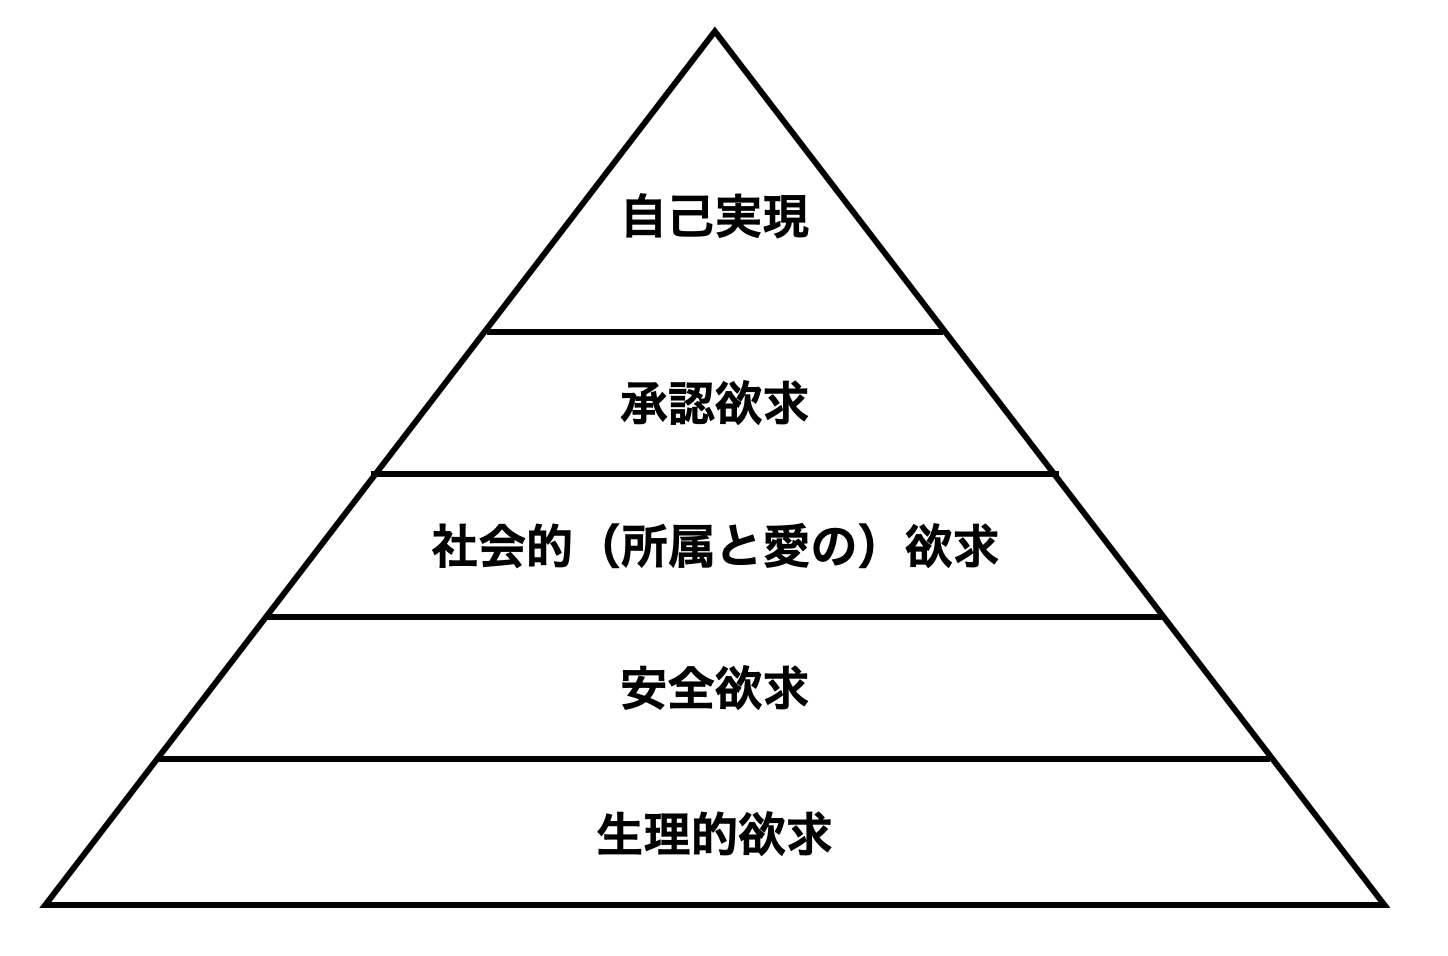
\includegraphics[keepaspectratio,width=0.7\linewidth]{../images/06_Maslow.png}
	\caption{マズロー\index[nameidx]{まずろー@マズロー}の欲求段階説のイメージ。この図もマズロー\index[nameidx]{まずろー@マズロー}が提案したものではありませんが，よく知られています。}
	\label{Maslow}
\end{figure}

重要なのは，人間は最終的に自己実現，つまり自分がなりたい自分になることをゴールとする存在だという考え方です。この根底には，人間は前向きで，ポジティブで，自己実現を目指す存在だという人間観があります。以前お話ししたかもしれませんが，精神分析\index[termidx]{せいしんぶんせき@精神分析}は無意識に捕らわれているとし，行動主義や認知心理学\index[termidx]{にんちしんりがく@認知心理学}的な発想は刺激と反応の関係で人間を説明する，いわばロボットのように人間を見る傾向がありました。これに対して，人間のポジティブな側面に注目したのがマズロー\index[nameidx]{まずろー@マズロー}です。

同様に，第三潮流のもう一人の提唱者であるロジャーズ\index[nameidx]{ろじゃーず@ロジャーズ}も，人間を無意識や環境の刺激に翻弄される存在としてではなく，自発的でポジティブな存在として捉えようとしました。ロジャーズ\index[nameidx]{ろじゃーず@ロジャーズ}は，クライエント中心療法を提唱した臨床家です。精神分析\index[termidx]{せいしんぶんせき@精神分析}では，相談者に対して「あなたは子供の頃にこういう欲求があったから，ここを直しなさい」とか，「こういうところに性的エネルギーがあるから，適切に発散させなさい」というような，非常にディレクティブ(指示的)な指導をします。そこには，無意識に支配される受け身的な人間像があります。

しかし，ロジャーズ\index[nameidx]{ろじゃーず@ロジャーズ}はそうではないと主張します。人間には本来ポジティブになろうとするエネルギーがあるのだから，「あれをしなさい，これをしなさい」と指示するのではなく，悩みを持つ人の話をそのまま受け入れ，よく聞くことが大切だと。これがノンディレクティブ，つまり指示性を持たない，受容と傾聴を中心としたカウンセリング方法として提案されたのです。

現代の臨床心理学の多くは，このロジャーズ\index[nameidx]{ろじゃーず@ロジャーズ}的な発想を基盤としていると考えられます。フロイト派の精神分析\index[termidx]{せいしんぶんせき@精神分析}は，カウンセラーとクライアントが何年も対話を重ねながら人格の抜本的な変革を目指す，時間とコストのかかるプロセスでした。一方，ロジャーズ\index[nameidx]{ろじゃーず@ロジャーズ}のクライエント中心療法は，定められた時間内でクライアントの話を聞くという，より手軽な方法です。これは良し悪しは別として，メンタルヘルスの相談をより身近なものにしたという実践的な意義があります。少なくとも，人間をポジティブに捉える視点を提供したという意味で，この第三潮流の影響は大きく，社会心理学\index[termidx]{しゃかいしんりがく@社会心理学}における人間観にも影響を与えました。

また，本テキストの著者である吉森先生が注目する方向性として，後期ウィトゲンシュタイン\index[nameidx]{うぃとげんしゅたいん@ウィトゲンシュタイン}の「言語ゲーム」という考え方があります。「言葉の意味とはその使用である」という発想で，言葉がどのようにやりとりされているかを重視します。これは，人が自分の人生をどう語るかという心理学的アプローチを生み出し，会話，コミュニケーション，言説の重要性を強調します。

これは「エスノメソドロジー\index[termidx]{えすのめそどろじー@エスノメソドロジー}」とも関連します。エスノメソドロジー\index[termidx]{えすのめそどろじー@エスノメソドロジー}は，一般的な社会というより，個々の現場での生活そのものをどう正しく解釈できるかを問うものです。客観的な科学的記述よりも，その生活や営みを行う人々の中に入り込んで参与観察することで，生き生きとした人間の営みを理解しようとするアプローチです。

これは必ずしも自然科学的ではありませんで，人文科学的なアプローチとして捉えることができるかもしれません。サイエンスなのか，人文学なのか，アートなのか，その境界は曖昧ですが，このような研究アプローチも生まれてきています。

\section{社会心理学は歴史の学か}

グループダイナミックス\index[termidx]{ぐるーぷだいなみっくす@グループダイナミックス}では，前回お話ししたようにアクションリサーチが基本方針でした。レヴィンは「良い理論ほど実践的なものはない」と述べ，基礎的な調査よりも現場の人の動きを科学的に考えることの重要性を説きました。レヴィンはまだ比較的予測と制御という科学的発想を持っていましたが，現代では予測や制御よりも説明と解釈に重きを置く研究スタイルも出てきています。このように，認知的な用語を使う論理実証主義\index[termidx]{ろんりじっしょうしゅぎ@論理実証主義}的アプローチ，ポジティブな人間観に基づく心理学的アプローチ，そして実践における意味や解釈を重視する社会学的枠組みなど，様々なアプローチが生まれてきたのです。

そんな中，1973年にガーゲン\index[nameidx]{がーげん@ガーゲン}が発表した``Social Psychology as History''が大きなインパクトを与えました。ガーゲン\index[nameidx]{がーげん@ガーゲン}は，社会心理学\index[termidx]{しゃかいしんりがく@社会心理学}は歴史の学なのだと主張したんですね。「実験をしているのだからサイエンスだ」というのがそれまでの社会心理学\index[termidx]{しゃかいしんりがく@社会心理学}の主流な考え方なんですが，ガーゲン\index[nameidx]{がーげん@ガーゲン}によれば，実験で扱っているのは人間の社会の極めて限定された一部分に過ぎず，実生活とは大きく乖離しているというのです。

重要なのは，私たちの日常生活のどの部分を切り取って「これが人間社会の姿だ」と言えるのか，という問いです。実験室のように条件を整えて，実験1，実験2，実験3と同じ条件で進められると考えること自体が誤りかもしれません。なぜなら，人間は皆それぞれの生活を持っており，環境や条件を整えたと言っても，厳密には全て異なる人が異なる経験をしているからです。つまり，自然科学のように「同じ結果が再現される」ということはありえないのです。

社会心理学\index[termidx]{しゃかいしんりがく@社会心理学}が行っているのは，時間の流れに沿って「その時点でこういう出来事があった」という歴史の記述に過ぎない，というのがガーゲン\index[nameidx]{がーげん@ガーゲン}の主張でした。この考え方は相当なインパクトがあり，社会心理学\index[termidx]{しゃかいしんりがく@社会心理学}者たちに「私たちはどんな学問をやっていたのか」「何をやりたかったのか」という根本的な問いを投げかけることになりました。

\subsection{社会的構築主義の考え方}
この流れから「社会的構築主義」という考え方が生まれてきます。これは，社会というものも結局は人々の信念体系が作り出している社会的実在\index[termidx]{しゃかいてきじつざい@社会的実在}に過ぎないという考え方です。社会とは何かと問うと，それは「みんなが社会があると思っている」ということに他ならない，というわけです。社会があって個人があるのではなく，社会とは個々人の共同幻想のようなものだという考え方です。

例えばお札がよく例として挙げられます。お札に価値があるのは，日本銀行券と書かれているからではなく，みんながそのお札に価値があると思っているから価値があるのです。仮に日本が財政破綻してデフォルトを起こした場合，どれほど立派な紙幣でも，ただの印刷された紙になってしまいます。1000円札が1000円の価値を持つのは，みんながそれを1000円相当のものと交換できると信じているからです。このように，社会とは全員の共有する考えの総体なのです。

つまり，社会は外在的・客観的に存在するのではなく，私たちが作り出しているものに過ぎないというスタンスで考える必要があるということです。社会心理学\index[termidx]{しゃかいしんりがく@社会心理学}が扱う「社会」も，実験室の中でみんながこれが「ここでの社会のやり方だろう」と思う雰囲気や空気のようなもの，つまりみんなの想定の総体に過ぎません。これも認知的な発想ですね。

ともかく，社会は頭の中のイメージの共有でしか存在しない，という発想が出てきたわけです。これを当たり前だと思う人もいれば，「社会とは政府や国家のことだ」というハードな立場の人もいるでしょうし，もう少し緩やかに「社会，国家，民族という確固としたものがある」と考える人もいるでしょう。社会構築主義的にいうなら，それらも認知の集合体として構築されているものであり，絶対的なものではなく，イメージの仕方次第で変わりうるものです。

さて，1970年代に，はっきりとした社会が客観的・外在的に存在するのではなく，「私たちが作っているものなのだ」という発想が出てきたことが，この転換期の重要なポイントとなります。これが先ほどの言語ゲーム，エスノメソドロジー\index[termidx]{えすのめそどろじー@エスノメソドロジー}，会話分析などと混ざり合って，ナラティブ研究，つまり人々が自分の社会をどう解釈し，どういうストーリーとして表現しているのかという研究方法につながっていくということです。

\section{ヨーロッパの社会心理学}
さて，この辺がアメリカの社会心理学\index[termidx]{しゃかいしんりがく@社会心理学}業界の中での動きだったわけですけれども，ここにちょっと別の流れも出てきます。ちょっとここでヨーロッパの方を振り返ってみましょう。ここまで，戦争による亡命などから重心がアメリカの方に来て，個人主義的，プラグマティックな社会心理学\index[termidx]{しゃかいしんりがく@社会心理学}っていうのが一つ完成したんでしたよね。

60年代，70年代，80年代になって，ヨーロッパの方でも少しずつ雰囲気が変わってきます。ヨーロッパ的な発想が出てくるわけですね。このヨーロッパ社会心理学\index[termidx]{しゃかいしんりがく@社会心理学}は，アメリカの社会心理学\index[termidx]{しゃかいしんりがく@社会心理学}に対して，社会学的な社会心理学\index[termidx]{しゃかいしんりがく@社会心理学}，あるいは個人主義的・プラグマティックなものとは違う，社会という全体的なエネルギーのようなものを重視する社会心理学\index[termidx]{しゃかいしんりがく@社会心理学}として展開されます。
\subsection{モスコビッチの少数派影響}
2つほど研究者及び理論を紹介したいのですが，1つはモスコビッチ\index[nameidx]{もすこびっち@モスコビッチ}というフランスの社会心理学\index[termidx]{しゃかいしんりがく@社会心理学}者です\footnote{セルジュ・モスコヴィッチ(Serge Moscovici, 1925年6月14日 - 2014年11月15日)は，ルーマニア生まれのフランスの社会心理学\index[termidx]{しゃかいしんりがく@社会心理学}者であり，特に「少数派影響」の理論で知られる。彼の業績は社会心理学\index[termidx]{しゃかいしんりがく@社会心理学}や政治心理学の分野で大きな影響を及ぼしている。(Wikipediaより)}。この人はテキスト的には社会的表象理論\index[termidx]{しゃかいてきひょうしょうりろん@社会的表象理論}という理論を展開したとされています。私はこの社会的表象理論\index[termidx]{しゃかいてきひょうしょうりろん@社会的表象理論}をあまりよくイメージできていないのですが，基本的に言いたいことは，社会的な文脈の中でないと物事は分からないということです。個人が実験室の中でどのように振る舞ったかということではなく，人間の社会的な文脈の中での意味合いの方が重要だという考え方です。

モスコビッチ\index[nameidx]{もすこびっち@モスコビッチ}の話で特に有名なのは，少数派の意見，マイノリティのインフルエンスについての研究です。以前，アッシュ\index[nameidx]{あっしゅ@アッシュ}の同調実験を紹介しましたよね。どういうものだったかというと，明らかに長さの違う棒を見て，標準刺激と比べてどれが長いかと聞かれた時，誰が見ても真ん中の長さだと分かっているのに，順番に全員が明らかに違う答えを言ってくる。それが自分の番に回ってくる。あなたは全体に同調せずに，その前の答え(サクラ，すなわち仕掛け人の嘘の答え)の圧力に負けずに，自分の考えを言えますか，という話です。

意見の対立があったときに，多数派と少数派を比べたら多数派の方が影響力が大きい，数が多い方が，声が大きい方が影響力が大きいというのは当たり前の発想です。しかし，モスコビッチ\index[nameidx]{もすこびっち@モスコビッチ}が言ったのは，少数派がしっかりと自分の意思や信念を持って，こちらの方が重要だということをずっと発信し続けていけば，いつかはそれが広がってマイノリティの意見が多数派の意見をひっくり返すこともある，そういうことも起こりうるのだということを，研究と共に紹介したのです。人間は必ずしも多数派に流されるばかりではないということ。実験室での短い時間で「はい，こういう影響がありました」で終わるのではなく，長いスパンの中で活動していくエネルギーが確実にあるということをモスコビッチ\index[nameidx]{もすこびっち@モスコビッチ}は主張したのです。

皆さんは「12人の怒れる男」\footnote{『12人の怒れる男』(12 Angry Men, 1957年)は，シドニー・ルメット監督によるアメリカ映画で，陪審員たちが少年の有罪か無罪かをめぐり議論を繰り広げる法廷ドラマである。物語は密室で行われ，偏見や感情にとらわれずに事実を見極めることの重要性が描かれている。映画は集団心理や意見の相違がどのようにして合意に至るかを探る優れた作品とされ，心理学や社会学の分野でも引用されることが多い。(Wikipediaより)}という映画をご存知でしょうか？ まだ見ていない方は，ぜひ見てください。とても良い映画です。もともとは白黒でしたが，カラー版にリメイクされ，さらに三谷幸喜が日本語版のパロディ映画を作るほど話題になった作品です。

この映画で重要なのは12人という人数で，これはアメリカの陪審員を指します。アメリカの裁判では，陪審員が「有罪か，無罪か」を決めます。結末を言ってしまうのは，これから見ようと思っている方には申し訳ないのですが…大丈夫でしょうか？ 言ってしまいますね。この映画では，圧倒的な多数派と少数派の対立が描かれます。「誰が見ても明らかだ，あの人は悪い。早く牢に入れるべきだ」という意見が多数派となりますが，ある人が「ちょっと落ち着いて考えてみよう。この点はどうだろう，あれはどうだろう」と続けて問いかけていくんです。すると徐々に少数派の意見も広まり，最初とは異なる雰囲気，結論に変わっていくという展開です。今，映画の結末を話してしまったかもしれません。しかし，この映画は単純なものではなく，密室での2時間弱の物語で，シナリオが濃密に書かれているので，結末を知っていても十分に楽しめます。ぜひ見てください。

このように，少数派の人でも影響力を持ちうるのです。そして実験室の中だけで全てが決まるわけではない，ということを主張したのですね。

\subsection{タジフェルの社会的アイデンティティ理論}
次に，タジフェル\index[nameidx]{たじふぇる@タジフェル}\footnote{アンリ・タジフェル\index[nameidx]{たじふぇる@タジフェル}(Henri Tajfel, 1919年6月22日 - 1982年5月3日)は，ポーランド生まれのイギリスの社会心理学\index[termidx]{しゃかいしんりがく@社会心理学}者で，特に「社会的アイデンティティ理論\index[termidx]{しゃかいてきあいでんてぃてぃりろん@社会的アイデンティティ理論}」の創始者として知られる。彼の研究は，集団間の偏見や差別のメカニズムを解明し，個人が所属する集団に対するアイデンティティが自己概念に与える影響を示した。(Wikipediaより)}の研究を紹介しましょう。タジフェル\index[nameidx]{たじふぇる@タジフェル}は「社会的アイデンティティ」という概念を提唱しました。

タジフェル\index[nameidx]{たじふぇる@タジフェル}の社会的アイデンティティ理論\index[termidx]{しゃかいてきあいでんてぃてぃりろん@社会的アイデンティティ理論}は，人間が自分を説明する際に社会的カテゴリーを使うという考え方です。例えば，Who am I テストという心理学の研究法があります。「I am XXX」という形で自己紹介を20個ほど書くのですが，皆さんならどう書くでしょうか。

私の場合であれば，「私は小杉です」「小杉考司です」「専修大学の教員をしています」「専門は社会心理学\index[termidx]{しゃかいしんりがく@社会心理学}と心理統計学です」というように，具体的なプロフィールを述べていきます。これは，自分が何者であるかを語る際に，所属している組織の名前や，所属している集団における社会的な位置を使って自分を説明していることを示しています。もちろん「僕はうどんとそばが好き」といった個人的な情報から始めることもできますが，多くの人は社会的カテゴリーから説明を始めます。私たちは自分がどういう社会的な立場にいるのかということに無意識的になっており，それによって自分をカテゴリー化しているのです。アメリカ的，個人心理学的な発想では「俺は俺だ！」で終わってしまいそうですが，実際には人間は社会的カテゴリーに応じて自分を説明します。つまり，社会的な背景を抜きにして個人を語ることはできないのです。人間は自分が何者なのかを社会的に定義することから始まる，という考え方が提案されました。

この社会的アイデンティティ理論\index[termidx]{しゃかいてきあいでんてぃてぃりろん@社会的アイデンティティ理論}は，ターナー\index[nameidx]{たーなー@ターナー}によってさらに自己カテゴリー理論として拡張されます。社会的カテゴリーは集団間の葛藤などがメインテーマですが，ターナー\index[nameidx]{たーなー@ターナー}の理論では，個人の中にそういった社会的な変数が入ってくるという考え方です。タジフェル\index[nameidx]{たじふぇる@タジフェル}とターナー\index[nameidx]{たーなー@ターナー}はイギリスの研究者ですが，ヨーロッパ的な視点から，個人が何者であるかということも重要だが，社会，環境，文脈を抜きにしては人間を語れないという心理学を展開していったのです。このように，アメリカで社会心理学\index[termidx]{しゃかいしんりがく@社会心理学}が盛り上がっていた時期に，ヨーロッパでは社会という文脈の中の人間という捉え方が出てきたということです。

\section{グループダイナミックスの変遷}
\subsection{レヴィンの理論とその後}
社会心理学\index[termidx]{しゃかいしんりがく@社会心理学}には様々なテーマが登場し，結果として混沌とした状況が生まれてきます。その原因は，社会心理学\index[termidx]{しゃかいしんりがく@社会心理学}の研究や考え方が10年，20年と時間が経つ中で多くの問題が明らかになってきたことです。もともと研究のスタイルや形式を確立しようとした人々の意図とメッセージが，いつの間にか「これが社会心理学\index[termidx]{しゃかいしんりがく@社会心理学}のやり方です」という形式的なハウツー論に変わり，本来の概念が正しく伝承されなかったからではないかと思います。

その具体例として，グループダイナミックス\index[termidx]{ぐるーぷだいなみっくす@グループダイナミックス}の話を見てみましょう。レヴィンが始めたグループダイナミックス\index[termidx]{ぐるーぷだいなみっくす@グループダイナミックス}は，生活空間や社会科学における場の概念，そしてその中での力学を考えるところまでは良かったのです。

しかし，問題点が二つありました。一つは，レヴィンが過労で早くに亡くなってしまい，彼のアイデアが構想段階で留まってしまったことです。もう一つは，レヴィンが提唱したトポロジー空間におけるダイナミックス，$B=f(P,E)$という式は格好良いのですが，その空間の特性が何なのか，場の理論であれば，場というフィールドの範囲や力，電磁場のようなものが何なのかという定義や説明がないまま，この式だけが残されてしまったことです。つまり「これは具体的に何なのか？」「どうやって研究すればいいのか？」という問題が残されたのです。

その背景には，レヴィンが生きていた時代の科学力，特に数学力の限界があります。彼の考えの基礎となる位相・トポロジー空間，位相数学\footnote{位相数学(トポロジー)は，図形や空間の形状を対象とする数学の一分野であり，連続的な変形(曲げたり伸ばしたりしても切断しない変形)において不変の性質を研究する。点集合の開集合系による空間の構造や，連結性，コンパクト性，位相同型といった概念が中心的に扱われ，物理学やデータ解析など様々な分野に応用される。特に「位相空間」や「基本群」の理論は位相数学の基本的な概念である。(Wikipediaより)}がまだ十分に発達していなかったのです。トポロジーで考えるというアイデアはあっても，「具体的にどうやるのか」という方法論が十分に確立されていなかったわけです。

そんな中，レヴィンの弟子たちはグループダイナミックス\index[termidx]{ぐるーぷだいなみっくす@グループダイナミックス}の研究をどう進めていったのか。レヴィンは，グループとはダイナミックな全体(A Dynamic whole)であり，そのメンバー同士が相互に依存していると述べ，その相互依存性の重要性を強調しました。相互依存性(inter-dependency)とは，メンバー同士が互いに存在の理由を持っているということです。グループの定義の仕方は他にも色々あります。例えば，目的達成のためにメンバーが集まっているとか，役割理論による説明があったりします。その中には，「このグループのメンバーになれば，ご飯が食べられるから，お金がもらえるから，うまくいくから，道具的に利用する」などの理由も含まれます。

しかし，レヴィン，あるいはモレノが考えていたのは，「お互いの存在をお互いに認めている」ということです。僕が存在する理由は，他の人が僕を認めてくれるからです。逆に，僕が他の人の存在を認めるからこそ，グループというものが形成されるのです。つまり，グループの中にいるメンバー同士は，互いの存在に依存しているのです。これを相互依存性と呼び，これがグループの本質だとレヴィンは語りました。

では，この相互依存性をどのように研究すればよいのでしょうか。レヴィンが考えた重要な特徴の一つが，集団凝集性\index[termidx]{しゅうだんぎょうしゅうせい@集団凝集性}(group cohesiveness)，つまりメンバーの結束の度合いです。

相互依存性，すなわちお互いの存在が互いに必要で，その上でどれだけ結束しているかということで，グループの特徴が描けるとレヴィンは考えていたようです。グループの中に止めようとする力，これが凝集性ですが，この結集力が重要なのです。例えば，グループのメンバーが「みんな，もっとグループとしてまとまろう」という力をかけるとします。この力の効果が最も顕著に表れるのは，実はグループの中心人物ではなく，グループの周辺にいる人たちなのです。「もしかしたらこのグループに入れないかもしれない」「私はこのグループのメンバーなのだろうか」「中心から離れているな」と感じている人ほど，コミュニケーションを取ろうとする圧力が強くかかると言われています。レヴィンのグループダイナミクスでは，グループとはそのように，みんながグループの中心の方に向かおうとする力学が生じるものだと説明します。

ちなみに，周辺メンバーの方がコミュニケーションに対するモチベーションが強くなるという指摘をしたのはフェスティンガー\index[nameidx]{ふぇすてぃんがー@フェスティンガー}です。レヴィンがこのことを知っていたかどうかは分かりません。なぜなら，その頃すでに亡くなっていたからです。

こうしたレヴィンの方針のもと，相互依存性あるいは集団凝集性\index[termidx]{しゅうだんぎょうしゅうせい@集団凝集性}を測定してサイエンスにしていこうという話になった時，お弟子さんたちはこの集団凝集性\index[termidx]{しゅうだんぎょうしゅうせい@集団凝集性}をどのように考え，どのように測定しようとしたのでしょうか。集団凝集性\index[termidx]{しゅうだんぎょうしゅうせい@集団凝集性}について，インタビューでも知られていないので，その測定方法の検討が重要なポイントとなったのです。

レヴィンのお弟子さんたちが考えた一つの答えは，この集団凝集性\index[termidx]{しゅうだんぎょうしゅうせい@集団凝集性}というのは集団に対する魅力である，ということですね。言葉を言い換えただけじゃないかと私は思うのですが，それは言わないでおきましょう。まあ，魅力であるというわけです。集団に対する魅力である。集団に対する魅力って何なのですか？と言われると，具体的には集団成員に対する魅力である。なんだかだんだん怪しくなってきていると思うのですが，集団メンバーに対する魅力です。集団に対する魅力というのは何かというと，とどのつまり，集団の成員，メンバーに対する魅力である。集団のメンバーに対する魅力というのはつまり，どういうことかというと，あのメンバーのことが好ましい，あのメンバーはかっこいい，このメンバーは素敵，このメンバーももっと頑張れみたいな。その人たちに，どれくらいいい人だなという印象をその人が持っているかということである。

さあ，このグループの凝集性を測定するにはどうしたらいいかというと，一人一人に，他のメンバーに対して，あなたはこの人に魅力をどれくらい感じていますか？あなたはこちらの人には魅力をどれくらい感じていますか？という集団の各メンバーに対する相互評定をすればいい。全員が他のメンバーに対して，いい人たち，魅力的な人たちと思っているグループと，そうでないグループを比べたら，明らかにその評定値が高いグループの方が魅力が高くて，集団に留まっていこうという力も強い。つまり集団凝集性\index[termidx]{しゅうだんぎょうしゅうせい@集団凝集性}が高いグループだと言えますね。言えますかね？言えますよね？という話になっていったわけです。

要するに，集団の凝集性を測定しましょうという話になったときに，集団の凝集性は集団の魅力，集団の魅力はメンバーの魅力，メンバーの魅力は対人魅力の相互評定だ。どうやって測定しますか？全員の対人魅力の評定値の相互評定だ。それの高いグループと低いグループを比べるんだ。という話になってますよね。

これって結局のところ，それが社会心理学\index[termidx]{しゃかいしんりがく@社会心理学}なの？というのが問題なのです。レヴィンが考えた，あるいはもっと広い意味でのゲシュタルト心理学\index[termidx]{げしゅたるとしんりがく@ゲシュタルト心理学}者の主張を思い出してみてください。「全体は部分の総和以上である」と言いましたよね。ゲシュタルト心理学\index[termidx]{げしゅたるとしんりがく@ゲシュタルト心理学}の発想ってそうなのです。部分を足したところで総和したって全体にはならないのです。でも，集団凝集性\index[termidx]{しゅうだんぎょうしゅうせい@集団凝集性}を測るのに総和でなくていい，対人魅力の相互評定なのだから，グループでなくなっちゃっているわけです。少なくともダイナミックな全体性ではなく，部分の総和にしかなっていないわけですね。この意味で，研究としての方向性がぶれているわけです。

そこをどうやってうまく，いや，「総和じゃないんだよ」って言えるのか，言えたのか，言えなかったのですね。グループダイナミクスの研究というのは，結局のところメンバー相互の印象評定の集計ということになった。これは，せっかく「個々人じゃないよ」って言っていたのが，個々人のレベルに戻ってしまったようなものなわけです。「グループというのは，そういう個々人の要素を足すだけじゃないのにね」って言っていたのが，こういう感じで崩れてきちゃいました。

\subsection{最小条件集団の衝撃}
タジフェル\index[nameidx]{たじふぇる@タジフェル}たちの社会的アイデンティティ理論\index[termidx]{しゃかいてきあいでんてぃてぃりろん@社会的アイデンティティ理論}，つまり私たちは自分たちの存在を社会的なカテゴリーで定義するという話から，もう一つ面白い研究が生まれました。それが「最小条件集団」という実験です。この実験はどのように行われるかというと，まず実験参加者を集めます。参加者は一人ずつ部屋に呼ばれていきます。部屋で実験者は2つの絵を見せます。これは抽象画なんです。そして「どちらの絵が好きですか？」と聞かれます。

私も絵心はないですし，美的なセンスも学識もありません。参加者の多くもそんな感じだったと思います。だから抽象画を見せられても，どちらが良いなんて分からないので，「何となくこちらが青っぽいので，こちらが好きです」とか，「何となくこちらが好きです」と，適当に答えると思います。抽象画は何でも良いのですが，2つの絵を見せて，どちらが好きかを選ばせるわけです。参加者が「私はこちらの絵が好きです」と言ったら，「では，あなたはこちらに。あなたは青色の絵を選びました。あなたは青色の絵を選んだグループのメンバーです」と言われます。

この青色の絵を選んだメンバーですが，この後，他にも青色の絵を選ぶメンバーが出てきます。出てくるとされている。そして参加者に言われるのは，これからもう一つの絵を選んだグループと，自分のグループとで，報酬を分け与えることになるのですが，「あなたの青色グループと向こうのグループで，報酬1万円を何対何に分けますか？」と聞かれる。そうすると，「自分は青色グループだから」と考えて，「では，青色グループが6000円で，あちらのグループが4000円，6対4くらいの割合で分けます」というように，自分が所属したグループにより多くの報酬を割り振るという現象が起きるのです。これは皆さんも同じようなことをしないでしょうか？

ここで重要なのは，自分が青色を選んだからといって，青色グループにたくさんの報酬を割り当てても，自分の得にはならないのです。というのも，「いや，あなたの報酬は別です。あなた以外の青色グループと，もう一つの絵を選んだグループとの間でお金を分配してください」と言われても，自分の報酬とは関係なく，自分が選んだ青色グループの方に多く割り振る傾向があるのです。なぜそんなことになるのか不思議です。だって，自分とは関係のない二つのグループなのだから，どちらでも良いはずです。しかも，自分が青色グループになった理由は，抽象画で適当に決めただけなんです。

この実験の面白いポイントは他にもあります。絵を選んだ時点では，まだグループになっているわけではありません。実験の部屋に別々に呼ばれて，「あなたはどちらの絵が好きですか？」「こちらです」という会話をしているだけなので，自分以外の青色グループにどんなメンバーがいるのかも分からない状態です。メンバー間の個人的なつながりは全くないのです。

例えば，とても魅力的な人が青色グループにいることが分かっていれば，自分の報酬と関係なくてもその人にたくさんお金をあげようと思うかもしれません。しかし，そういった要素も全くありません。誰がメンバーか分からないし，自分の利得にも関わらないのに，実験をすると明らかに自分が選んだグループの方を高く評価するのです。タジフェル\index[nameidx]{たじふぇる@タジフェル}らが言うように，これは社会的カテゴリーで自分を定義するからなのです。具体的な中身は伴っていなくても構いません。カテゴリーとして「私は青色グループだ」という認識があれば，それだけで行動が変容するという話です。

この話のテーマが「最小条件集団」という名前からも分かるように，集団，グループとは一体何なのか？ 「青色グループ」とは一体何なのか？ というと，タジフェル\index[nameidx]{たじふぇる@タジフェル}に言わせれば，それは「青色グループ」というカテゴリーが存在すること，それだけの枠があるだけなのだという話です。自分が青色のグループ，もう一つがそれ以外のグループとなると，自分のグループに有利に，相手のグループが不利になるように。自分のグループのメンバーは個性豊かで立派な人たち，自分以外のグループは何か無機質で，均一的で，無能な，ちょっと劣った人たちと勝手に意味付ける。この分け目が生まれるのは何かというと，ただ分けただけなのです。分けるということがグループを生むのだという話を社会的カテゴリー理論はしたのです。

これが「最小条件」というのは，グループを作る最小の条件とは何かというと，カテゴリーがあることだけ，とするからです。分けたという事実だけなのです。これはそれまでのグループダイナミクスをはじめとするグループの研究に大きなインパクトを与えました。先ほども言ったように，グループというのは，何か集団としての目的があるから，集団の目的に賛同して集まっているのだ，あるいはこの集団にいることでメリットがあるから所属しているのだ，という形で集団を定義する人がいました。あるいはモレノやレヴィンのように，メンバー同士の相互の存在の強さ，ソーシャルボンドの強さ(モレノは「テレ」という，感情の流れを指す言葉を使います)，その情緒的なつながりとか，存在を相互に依存し合っているからグループというのがあるのだという話をしているのですが，先ほどの実験の中にそんなものはどこにもありません。青色グループが目指すべきゴールもないし，青色グループにいたから得をするかというと，その人の給料は別ですと言われているのですから，別にそのグループにいたから得するわけでもない。メンバーを誰も見たことも聞いたこともないのですから，情緒的なつながりもなければ，相互に依存もしていない。だけど，グループに分けたということによる行動の変容，つまり全く平等な分割を行わないのです，人間は。内集団びいきという事実が発生する，グループに所属しているということによる効果が発生する。グループというのはカテゴリーなのですよ，という話が出てきたわけです。これに対して，集団心理学，グループダイナミクスの人たちが正しく，理論的に反論したかというと，残念ながら私はその反論を知りません。皆さんはうまく反論できるでしょうか?

レヴィンのお弟子さんたちは集団の要素，相互依存性のようなものを結局，総和の足し算に落とし込んでしまいました。一方，ヨーロッパからは，結局グループとは「グループがある」と言ったものに過ぎず，メンバーのことなど考える必要もないという話になってしまいました。このようなことから，グループダイナミクスは徐々にグループでもダイナミクスでもなくなっていき，社会心理学\index[termidx]{しゃかいしんりがく@社会心理学}の一ジャンルである対人魅力や，実験における社会的刺激としての「あなたはAグループ，Bグループ」といった枠組みに縮小してしまい，それ以上のものが出てこなくなってしまったように思います。

私が98年に大学院生になった時，社会心理学\index[termidx]{しゃかいしんりがく@社会心理学}会とグループダイナミクス学会に入会しました。その時すでに同期や先輩たちと，このグループダイナミクス学会はあと何年持つだろうかという話をしていました。というのも，もはやグループでもダイナミクスでもないし，社会心理学\index[termidx]{しゃかいしんりがく@社会心理学}会とやっていることは同じ。それどころか，社会心理学\index[termidx]{しゃかいしんりがく@社会心理学}会より会員数が少なく，学会の規模も小さい。社会心理学\index[termidx]{しゃかいしんりがく@社会心理学}会の中に内包されるような形でグループダイナミクス学会があり，その存在意義はどこにあるのかということが，院生レベルでも十分囁かれていました。私も，そのうちこの学会は潰れるだろうと勝手に思っていましたが，幸いにして，あるいは幸いかどうかわかりませんが，まだ残っています。

ただ，なぜ私たち院生レベルでもそのように考えていたかというと，スタート時のレヴィンが語った力強いグループ，集団，力学，相互依存性，サイエンスというエネルギーが，徐々に技術的に洗練されていき，ハウツーになっていき，あるいはさらに言えば測定，分析が高度になっていったということもあって，グループということ自体，あるいはダイナミクスと呼べるほどのダイナミクスを誰も研究できなくなっていったという実態があるのではないかと思います。

この授業は講義録を取っていて，一応記録として公開しようと思っているのですが，この記事をグループダイナミクス学会の人に読まれたら，非常に叱られるかもしれないと思っています。でも，まあ，いいでしょう。もし本当にグループダイナミクス学会がグループダイナミクスをちゃんとやってくれるのであればいいのですが，少なくとも一介の研究者にこのようなことを言われる程度に弱ってきているというのは事実としてあったということを覚えておいてください。

皆さんはグループダイナミクスあるいはグループというものを，社会心理学\index[termidx]{しゃかいしんりがく@社会心理学}の一部として考えていただいて構いません。ただし，社会心理学\index[termidx]{しゃかいしんりがく@社会心理学}が発展していく一方で，グループダイナミクスが弱っていくという時代の流れは知っておいていただきたいと思います。私は日本国内の事情しか知りませんが，世界的にはグループダイナミクス学会の参加者は多いかもしれません。少なくとも日本の学会においては，グループダイナミクス学会の方が歴史は古いものの，現在は学会の規模としては社会心理学\index[termidx]{しゃかいしんりがく@社会心理学}会よりも小さくなってきています。社会心理学\index[termidx]{しゃかいしんりがく@社会心理学}会は発足こそグループダイナミクス学会より後ですが，現在では会員数は増加を続け，社会心理学\index[termidx]{しゃかいしんりがく@社会心理学}という一つの学問のメンバーを抱えている状況です。この授業は社会心理学\index[termidx]{しゃかいしんりがく@社会心理学}の講義なので社会心理学\index[termidx]{しゃかいしんりがく@社会心理学}の話が中心ですが，グループダイナミクスという分野が存在した(まだなくなってないですけど)ことは覚えておいてください。

\section{いんたーみっしょん；科学の終焉}
これで私の話は現代に近づいてきました。

では，話の筋を変えて，残り15分ほどですので，今週の読書案内として面白い本を紹介したいと思います。それは「科学の終わり」\parencite{theEndOfScience}という本で，ジョン・ホーガン\index[nameidx]{ほーがん@ホーガン}が書き，筒井康隆が監修しています。1996年の出版です。この本は「科学は終わったのではないか？」という問いを投げかけています。特に進化論と相対性理論\index[termidx]{そうたいせいりろん@相対性理論}以上の大きな理論は発見されていないと指摘します。科学というのはもう大きな理論の発見が終わり，小さな未確認の事象を拾い続けるだけなのではないか，というのがその主張です。

社会心理学\index[termidx]{しゃかいしんりがく@社会心理学}はどうでしょうか？大きな問題を見据えて，理論を打ち立てたと言えるでしょうか。私の見立てでは，まだそこまで至っていないと思います。社会心理学\index[termidx]{しゃかいしんりがく@社会心理学}には公理のようなものはなく，時代と共に現れる新しい社会的な刺激に対する人々の考えを次々と集めているだけです。小さな理論の寄せ集め，今あるホットトピックを追いかけているだけかもしれません。このテキスト，アナトミア\parencite{anatomia}の方でも，社会心理学\index[termidx]{しゃかいしんりがく@社会心理学}者が追いかけている問題って一体何なのか，大統一理論のようなものがなくなって，細かい穴だけを集めているのではないか，という批判も紹介されてます。

社会心理学\index[termidx]{しゃかいしんりがく@社会心理学}では，レヴィンの場の理論も，それ以上の精緻化を試みる人はほとんど現れていません。むしろ，レヴィンの理論は忘れ去られたような状態です。レヴィンはトポロジーやダイナミクスといった専門用語を使用していましたが，中身が伴っていなかったのではないかという批判さえあります。

これをどう解釈するか，本当に天才的だったが時代や技術が追いついていなかったのか，それとも中身が伴っていなかったのか，その判断は皆さんに委ねたいと思います。現代の科学も，これ以上の大きな発展はないのかもしれません。この本では「知能や科学の終わり」と書かれていますが，これも一つの見方として考慮に値するでしょう。

\section{新しい研究アプローチの登場}
\subsection{計算機の発展と影響}
さて，長く話してきましたが，2000年代からの社会心理学\index[termidx]{しゃかいしんりがく@社会心理学}の危機については，時間が足りないので次回に譲りたいと思います。この危機は現代にも関わってきますし，私の専門領域とも関連が深いので，じっくりと詳しく話すつもりです。
残りの時間は，このテキストが2000年までの関東以外の社会心理学\index[termidx]{しゃかいしんりがく@社会心理学}について触れていないので，その頃を生きていた私の体験談をお話ししたいと思います。社会心理学\index[termidx]{しゃかいしんりがく@社会心理学}の業界でグループダイナミクスが活発だったという話はしましたが，90年代後半からの社会心理学\index[termidx]{しゃかいしんりがく@社会心理学}で何が起きていたのかをお話しします。

まず触れなければならないのが，コンピュータの進化です。TSSの話は既にしましたが，大型コンピュータからパーソナルコンピュータへのダウンサイジング，そして通信技術やコミュニケーション技術が徐々に広がっていきました。1995年にはWindows95が登場し，これによってパソコンが一般家庭に普及しました。それまでは，パソコンを購入するとOSがワンセットで付属していて，それがビルトインされているのが基本でした。しかし，ハードウェアとOSが別々に販売されるようになり，ハードウェアがDOS/Vという一般的な互換機\footnote{DOS/Vは，IBMが1990年に発表したPC/AT互換機向けの日本語対応OSの規格であり，日本語の表示や入力を可能にする技術である。当時，日本市場では専用の日本語処理ボードが必要だったが，DOS/Vにより標準ハードウェアで日本語を扱えるようになり，日本のPC市場に大きな変革をもたらした。(Wikipediaより)}の形状を持っていれば，Windows95をインストールできるということで，様々なメーカーがパソコンを製造し，Windows95で動作するようになりました。

その時代とほぼ同時期に，インターネットが広まります。インターネットは，元々はアメリカの軍事ネットワークであるARPANETから始まりました\footnote{ARPANET(アーパネット)は，1969年にアメリカ国防総省の高等研究計画局(ARPA)によって開発された世界初のパケット通信ネットワークであり，インターネットの前身とされる。ARPANETは分散型ネットワーク構造を採用し，ノード間で情報が効率的に転送される仕組みを導入した。研究機関や大学を中心に接続され，1970年代から1980年代にかけて広がり，現代のインターネット技術の基礎を築いた。(Wikipediaより)}。これが軍事的な連絡手段から，科学者同士が研究論文を交換するネットワークになり，その後は一般のネットワークやテレネットワークという形で広まり，インターネットとなったのです。僕が初めてインターネットの画面を見たのは，96年の冬ごろでした。その頃に僕はプロバイダと契約し，初めてインターネットを使ってみました。当時はNASAのホームページなどを見て，リアルタイムで外国の企業のサイトが見られるという事実に驚いたものです。

さらに94年と言えば，ポケットベルが流行っていました。皆さんにはあまり馴染みがないかもしれませんが，これは業務連絡用の小型のベルです。営業員が外出中でも，会社からの連絡を受け取るために使われていました。そのポケットベルにメッセージ機能が付くと，文字が送れるようになりました。最初は，ベルが鳴ったら会社に連絡するだけでしたが，ベルが鳴った時に誰からの連絡か，あるいは短いメッセージが送られるようになったのです。そして，それが女子高校生などを中心に，リアルタイムで電話でメッセージをやり取りするものとして流行っていました。なので，1994年の頃は，お昼休みになると公衆電話の前に行列ができていました。みんな10円玉を握りしめて，あるいはテレカ\footnote{テレホンカードは，主に公衆電話での通話料金を前払いするために使われるプリペイドカード。1982年に日本で初めて導入され，全国の公衆電話で利用可能となった。カードには磁気ストライプがあり，利用ごとに残額が減少する仕組み。通信インフラの発展と共に利用は減少したが，コレクターアイテムとしても人気がある。(Wikipediaより)}を準備して，電話をかけながら情報をやり取りする時代でした。

その後，PHS\footnote{PHS(Personal Handy-phone System)は，1990年代に日本で開発された携帯電話システムで，家庭用コードレス電話と携帯電話の中間的な役割を持つ。小型で低消費電力，音質が良いことが特徴で，主に都市部で利用された。通信コストが比較的安価で，ビジネス向けのサービスとしても普及したが，スマートフォンやLTEの普及により2020年代にはほとんど使われなくなった。(Wikipediaより)}や携帯電話が出てきました。ただ，携帯電話から携帯電話に電話をかけるだけでなく，メールも送れるようになったのです。そして，音声を送れるようになり，写真や動画も送れるようになりました。昔の人と会話すると，携帯で写真を送ることを「シャメを送る」と言う人がいるかもしれませんが，これは当時の商品名で，「写メ」は写真のメールが送れるという意味でした。

何が言いたいかというと，コミュニケーションデバイスが大きく発展たということです。かなり急激なスピードで，ですね。そして，それによってComputer Mediated Communicationという新しいコミュニケーションのスタイルが現れた。2チャンネルなどの掲示板，BBSのスタイルや，ブログ(ウェブログ)による情報公開があって，これはなんだ，なんでそんなことをするんだ，ということで社会心理学\index[termidx]{しゃかいしんりがく@社会心理学}でも自己開示，自己提示などの概念とともに研究され始めたのです。人間の社会的な関係を研究するのももちろん社会心理学\index[termidx]{しゃかいしんりがく@社会心理学}の一部ですが，社会的な刺激，社会的な技術，ネットが出てきたことは世界が大きく変わるほどの変化でした。そのため，コミュニケーションの取り方が大きく変わった時，人間はどうなるのかという研究テーマが生まれました。

\subsection{ゲーム理論とシミュレーション研究}
コンピューターの発展により，社会心理学\index[termidx]{しゃかいしんりがく@社会心理学}の中で新しい考え方が注目されるようになりました。それは，進化心理学的な発想や進化シミュレーションの考え方です。これはゲーム理論\index[termidx]{げーむりろん@ゲーム理論}を基に始まりました。

ゲーム理論\index[termidx]{げーむりろん@ゲーム理論}とは，プレイヤーが有限の手数とルールを知っている状況で，最適な行動を選択する理論です。この理論をコンピューターで実行することで，新たな発見がありました。ロバート・アクセルロッド\index[nameidx]{あくせるろっど@アクセルロッド}は，『つきあい方の科学』という本\parencite{Axelrod}の中で，このシミュレーションについて説明しています。彼は，相手を裏切ると得点が高くなるが，お互いに裏切り合うと最も損をするというゲーム構造を研究しました。

この「繰り返し囚人のジレンマゲーム」を繰り返すと，長期的には協力する方が有利だということが分かります。一回限りのゲームでは裏切る方が得ですが，長く繰り返すゲームでは協力する方が良いのです。この協力戦略，つまり長期的な繰り返しゲームにおいて，どのアルゴリズム，どの戦略を選べば強いのかというシミュレーション研究です。繰り返し囚人のジレンマゲーム大会で，最強の戦略を全米で募集したところ，優勝したのは心理学者\footnote{アナトール・ラパポート\index[nameidx]{らぱぽーと@ラパポート}(Anatol Rapoport, 1911年5月22日 - 2007年1月20日)は，ロシア生まれのアメリカの数学者，心理学者，ゲーム理論\index[termidx]{げーむりろん@ゲーム理論}家であり，特に「協力の進化」や「戦略的相互作用」に関する研究で知られる。彼は，囚人のジレンマにおける協力行動のモデル化や「タイタ・フォー・タット」戦略の提唱に貢献した。ラパポート\index[nameidx]{らぱぽーと@ラパポート}の研究は，平和学や国際関係の分野にも影響を与えた。(Wikipediaより)}の書いたTit for Tat(しっぺ返し)戦略でした。しかも，それは最も短いプログラムだったと言われています。相手が出した手を次のターンで同じように返す，つまり相手が協力してきたら協力して返し，裏切ってきたら裏切り返すという戦略が最強だということが分かったのです。

このような研究から，社会関係や協力行動が進化的に形成されてきたのではないかという説明をする研究者が現れました。社会心理学\index[termidx]{しゃかいしんりがく@社会心理学}における進化心理学派は，2000年代には人気を集めていたと思います。特に北海道大学にいた山岸先生とそのお弟子さんたち，私なんかは「北大一派」と呼んでましたが，進化心理学的な視点から，社会は協力し合った方が得をするような形に進化してきたという説明をするようになりました。

この研究の面白い点は，コンピューターでシミュレーションを行い，各戦略がどのような結果をもたらすかを理論的な最適化として示せることです。さらに，人間を使った実験室実験の結果と比較することで，理論と実際の人間行動とのギャップ，つまり理論的には協力した方が良いのにそうしない場合など，そのずれこそが心理学が考えるべき領域だと示すことができます。このような進化心理学的な社会心理学\index[termidx]{しゃかいしんりがく@社会心理学}が登場したのが2000年頃だと理解しています。興味のある方は，山岸俊男教授の『信頼の構造』という本\parencite{Yamagishi}を読んでみてください。非常に分かりやすい本です。

この時代は，コンピュータを使った研究がコミュニケーションの世界や社会的な理論の説明にも導入された時期です。また，統計技術も大きく進歩し，98年頃には回帰分析，因子分析などを統合する構造方程式モデリングが登場するなど，技術の進歩が社会心理学\index[termidx]{しゃかいしんりがく@社会心理学}の重要なポイントとなってきました。この統計的な技術の進歩と，2011年に起こった社会心理学\index[termidx]{しゃかいしんりがく@社会心理学}における再現性\index[termidx]{さいげんせい@再現性}の危機については来週お話しし，歴史シリーズを終えたいと思います。

なお，LMSでコメントを受け付けていますので，ご意見があればぜひ投稿してください。また，課題も出ていますので，必要な方はチャレンジしてください。では今日の話はここまでにしておきましょう。

\printbibliography[title=引用文献]

\end{document}

